\section{Normalization of \ac{t2w}-\ac{mri} images} \label{sec:chp5:T2-norm}

This section focuses on \ac{t2w}-\ac{mri} normalization.
First, the related work is presented in \ac{sec}\,\ref{subsec:chp5:relwork1} before to focus on two new normalization methods which are presented and investigated in \acs{sec}\,\ref{subsec:chp5:T2-norm:meth} and \acs{sec}\,\ref{subsec:chp5:T2-norm:Exp-res}

\subsection{Related work}\label{subsec:chp5:relwork1}

We briefly recall the state-of-the-art methods which have been proposed for the normalization of \ac{t2w}-\ac{mri} prostate images.

\citeauthor{Artan2010}, \citeauthor{Ozer2010}, and \citeauthor{rampun2016computerb} used a parametric method to normalize \ac{t2w}\ac{mri} images~\cite{Artan2009,Artan2010,Ozer2009,Ozer2010,rampun2015classifying,rampun2015computer,rampun2016computer,rampun2016computerb}.
This parametric method is based on computing the standard score --- also known as \emph{z-score} --- of the \ac{pz} voxels such as: 
\begin{equation}
  I_{s}(x) = \frac{I_{r}(x) - \mu_{PZ}}{\sigma_{PZ}}, \forall x\in PZ ,
  \label{eq:zscore}
\end{equation}
\noindent where, $I_{s}(x)$ and $I_{r}(x)$ are the standardized and the raw signal intensity, respectively, and $\mu_{PZ}$ and $\sigma_{PZ}$ are the mean and standard deviation of the \ac{pz} signal intensity, respectively. 
This transformation enforces the image \ac{pdf} to have a null mean and a unit standard deviation.
However, this normalization is not appropriate if the \ac{pdf} do not follow a Gaussian distribution as illustrated in Fig.\,\ref{fig:fitting}

\citeauthor{Lv2009}~cite{Lv2009} used the non-parametric method which is a piecewise-linear normalization, proposed by \citeauthor{Nyul2000} in~\cite{Nyul2000}.
For a given patient, a warping function is inferred by matching some specific landmarks --- i.e., different percentiles --- of the current \ac{pdf} to the same landmarks learned during a training phase from several patients. 
The mapping between each landmark is performed using a linear mapping.
\citeauthor{Viswanath2012} used a variant of the previous method by segmenting first the image using region growing with a pre-defined homogeneity criterion and keeping only the largest region to build the \ac{pdf}~\cite{Viswanath2012}.
Nevertheless, the warping functions inferred by these methods suffer from abrupt changes --- refer to \acs{fig}\,\ref{fig:maplinear} --- around the landmarks position, leading to a disrupt \ac{pdf} in the normalized image.

In this section, we evaluate and compare different normalization approaches in the context of \ac{t2w}-\ac{mri} prostate image normalization.
Our contribution is threefold: (i) a parametric normalization approach based on a Rician \textit{a priori}; (ii) a non-parametric normalization approach based on a method used in registration of functional data; and (iii) a novel evaluation metric to asses quantitatively the alignment of the \acp{pdf} independently of the assumed distribution. 
These methods are compared qualitatively and quantitatively, with both \textit{z-score} normalization and piecewise-linear normalization.

\subsection{Methodology}\label{subsec:chp5:T2-norm:meth}

\subsubsection{Parametric normalization using Rician \textit{a priori}}\label{subsubsec:chp5:T2-norm:meth:rician}
As previously stated, proper normalization of the \ac{mri} data during pre-processing is a key problem that has been addressed using parametric and non-parametric strategies.
We believe that normalizing \ac{mri} data using a parametric model based on a Rician distribution would improve the results.
Expecting this improvement by changing the data model from the widely used Gaussian distribution to Rician distribution is reasonable.
Indeed, \citeauthor{Bernstein1989} state that \ac{mri} data theoretically follow a Rayleigh distribution for a low-\ac{snr} scenarios while it appears closer to a Gaussian distribution when the \ac{snr} increases~\citeauthor{Bernstein1989}.
Figure~\ref{fig:fitting} shows the intensity spectrum for some \ac{mri} prostate data as well as the fitted Gaussian and Rician distributions.
A qualitative assessment of the underlying distribution is performed by overlying the fitted distribution, while quantitative results of the fitting are given in terms of \ac{rms}.
It can be highlighted that the Rician model better fits the data than the Gaussian model.

\begin{figure}
  \centering
  \subfigure[]{
    \label{fig:p1}\includegraphics[width=0.48\textwidth]{5_normalization/figures/T2-normalization/03}}\hfill
  \subfigure[]{
    \label{fig:p2}\includegraphics[width=0.48\textwidth]{5_normalization/figures/T2-normalization/06}}\hfill
%  \subfloat[][]{
%    \label{fig:p3}\includegraphics[width=0.3\textwidth]{14}}
  \caption{Visual evaluation of the goodness of fitting using Rician and Gaussian distribution.}
  \label{fig:fitting}
\end{figure}

The normalization is carried out through the following 3 steps: 
(i) fit a Rician model --- \acs{eq}\,\eqref{eq:rice} --- to each prostate \ac{pdf} using non-linear least squares minimization, namely Levenberg-Marquardt; 
(ii) compute the mean --- \acs{eq}\,\eqref{eq:meanr} --- and variance --- \acs{eq}\,\eqref{eq:var} --- of the Rician model;
(iii) normalize the entire data using the \textit{z-score} similarly as in~\acs{eq}\,\eqref{eq:zscore}.

\begin{equation}
  f(x| \nu, \sigma) = \frac{x}{\sigma^2}\exp\left( \frac{- (x^2 + \nu^2)}{2\sigma^2} \right) I_0 \left( \frac{x \nu}{\sigma^2} \right) \ ,
  \label{eq:rice}
\end{equation}

\begin{equation}
  \mu_{r} = \sigma  \sqrt{\frac{\pi}{2}}\,\,L_{1/2}(-\frac{\nu^2}{2\sigma^2})  \ ,
  \label{eq:meanr}
\end{equation}

\begin{equation}
  \sigma_{r} = 2\sigma^2+\nu^2-\frac{\pi\sigma^2}{2}L_{1/2}^2\left(\frac{-\nu^2}{2\sigma^2}\right)  \ ,
  \label{eq:var}
\end{equation}

\noindent where $\nu$ and $\sigma$ are the distance between the reference point and the center of the bi-variate distribution and the scale, respectively; $L_{1/2}$ denotes a Laguerre polynomial; $I_0$ is the modified Bessel function of the first kind with order zero.

\subsubsection{Non-parametric normalization based on \acs*{srsf}}\label{subsubsec:chp5:T2-norm:gen-model}

\citeauthor{Srivastava2011} proposed a generic method to register functional data, without any assumption regarding the models of the different functions~\cite{Srivastava2011}. 
In a nutshell, this framework relies on the \ac{srsf} representation which transforms the Fisher-Rao metric into the conventional $\mathbb{L}^2$ metric, and thus allows to define a cost function corresponding to an Euclidean distance between 2 functions in this new representation.

\paragraph{\Ac{srsf} representation}

In the proposed registration framework of functional data, 2 functions $f_1$ and $f_2$ are registered by composing $f_2$ with a warping function $\gamma$ such that:

\begin{equation}
  \argmin_{\gamma \in \Gamma} D_{FR}(f_1, (f_2 \circ \gamma)) \ ,
  \label{eq:regfun}
\end{equation}

\noindent where $D_{FR}$ is the Fisher-Rao distance and $\Gamma$ is the set of all the functions $\gamma$.

The \ac{srsf} representation is used to transform the functions and register them into this space.
The \ac{srsf} of a function $f$ is defined as:

\begin{equation}
  q(t) = \sign(\dot{f}(t))\sqrt{|\dot{f}(t)|} \ ,
  \label{eq:srsf}
\end{equation}

\noindent where $\dot{f}(t)$ corresponds to the derivative of $f$.

The major property of the \ac{srsf} representation used in the registration framework is the following: the composition of a function $f$ with a warping function $\gamma$ --- i.e., $f \circ \gamma$ --- is equivalent to \acs{eq}\,\eqref{eq:warp}, using the \ac{srsf} representation.

\begin{equation}
  \tilde{q}(t) = (q(t) \circ \gamma) \sqrt{\dot{\gamma}} \ ,
  \label{eq:warp}
\end{equation}

\noindent where $\dot{\gamma}$ is the derivative of $\gamma$.

Using this property, a cost function --- so called amplitude or $y$-distance --- is defined to measure the similarity between the 2 functions $f_1$ and $f_2$, expressed as in \acs{eq}\,\eqref{eq:cf}

\begin{equation}
  D_y(f_1, f_2) = \underset{\gamma \in \Gamma}{\infspie} \| q_1 - (q_2 \circ \gamma) \sqrt{\dot{\gamma}} \| \ .
  \label{eq:cf}
\end{equation}

\paragraph{Registration framework}\label{par:chp5:T2-norm:regfra}

The registration framework consists of 2 steps.
First, an initialization in which the Karcher mean $\mu_f$ is computed as in \acs{eq}\,\eqref{eq:mean}

\begin{equation}
  \mu_f = \argmin_{f \in \mathcal{F}} \sum_{i = 1}^{n} D_y(f, f_i)^2 \ .
  \label{eq:mean}
\end{equation}

Then, for each function $f_i$: 
(i) compute $\gamma_{i}^{*}$ as in \ac{eq}\,\eqref{eq:warpi}; 
(ii) compute $\tilde{q}_i$ as in \ac{eq}\,\eqref{eq:warp};
(iii) update $\mu_f$ as in \ac{eq}\,\eqref{eq:mean} by replacing $f_i$ by $\tilde{f_i}$, using $\tilde{q}_i$.

\begin{equation}
  \gamma_{i}^{*} = \argmin_{\gamma \in \Gamma} \sum_{i = 1}^{n} D_y(\mu_f, f_i)^2 \ ,
  \label{eq:warpi}
\end{equation}

\noindent where $n$ is the total number of functions to be aligned.

This step is performed in an iterative manner based on the gradient of the cost function given in \acs{eq}\,\eqref{eq:mean}. 
We refer the reader to the work of \citeauthor{Srivastava2011} for more detailed discussion~\cite{Srivastava2011}.

\subsubsection{Evaluation metric}

In their work, \citeauthor{Nyul2000} evaluated the normalization methods by computing the variation of the mean of a specific tissue.
However, this measure can be biased since that the mean can also be used as a landmark with the piecewise-linear method.
Furthermore, considering a single statistic does not allow to evaluate the overall performance of a normalization.
Indeed, this statistic corresponds to evaluate a single point of the mapping function and thus a large portion of the mapping functions are disregarded. 

That is why, to evaluate the performance of the different metric, we propose to use a spectral evaluation by decomposing the set of normalized \ac{pdf}s using \ac{pca} under the assumption that they are linearly dependent. 
Intuitively, the eigenvalues of the \ac{pca} decomposition are correlated with the alignment of the different \acp{pdf}.
Thus, in the case of a perfect alignment of the \ac{pdf}s, the first eigenvalue is much greater than the remaining since that the first eigenvector encodes all the information.
In the contrary, in the case of a misalignment of the \ac{pdf}s, more eigenvectors are needed to encode the information synonymous with larger eigenvalues.
Therefore, the cumulative sum of the normalized eigenvalues as well as the \ac{auc} are used, as depicted in \acs{fig}\,\ref{fig:qt}.

\subsection{Materials}\label{subsec:chp5:T2-norm:Exp-res}

The experiments are conducted on a subset of the public \ac{mpmri} prostate presented in \acs{sec}\,\ref{chp4:sec:data}.
We used the \SI{3}{\tesla} dataset which is composed of a total of 20 patients of which 18 patients had biopsy proven \ac{cap} and 2 patients are ``healthy'' with negative biopsies. 
In this study, our subset consists of 17 patients with \ac{cap}.

The different normalization methods are implemented in Python and are part of the \texttt{protoclass} toolbox presented in \acs{sec}\,\ref{chp4:sec:data}.
The normalization based on \ac{srsf} uses the implementation\footnote{\url{https://bitbucket.org/tetonedge/fdasrsf}} of \citeauthor{Tucker2013}~\cite{Tucker2013}.
The piecewise-linear normalization is performed using the following set of percentiles $s \in \{0, 5, 25, 50, 75, 95, 100 \}$ as landmarks.
In the \ac{srsf}-based normalization, the \acp{pdf} are smoothed using spline-based denoising method.

\subsection{Results and discussion}

\paragraph{Qualitative results}

% \begin{figure}
%   \centering
%   \includegraphics[width=1.\textwidth]{5_normalization/figures/T2-normalization/qualitative.png}
%   \caption{Qualitative evaluation by visual inspection of the alignment of the \ac{pdf}s for the full prostate and the \ac{cap}.}
%   \label{fig:qu}
% \end{figure}

\begin{figure}
  \hspace*{\fill}
  \subfigure[Piecewise-linear mapping function.]{
    \label{fig:maplinear}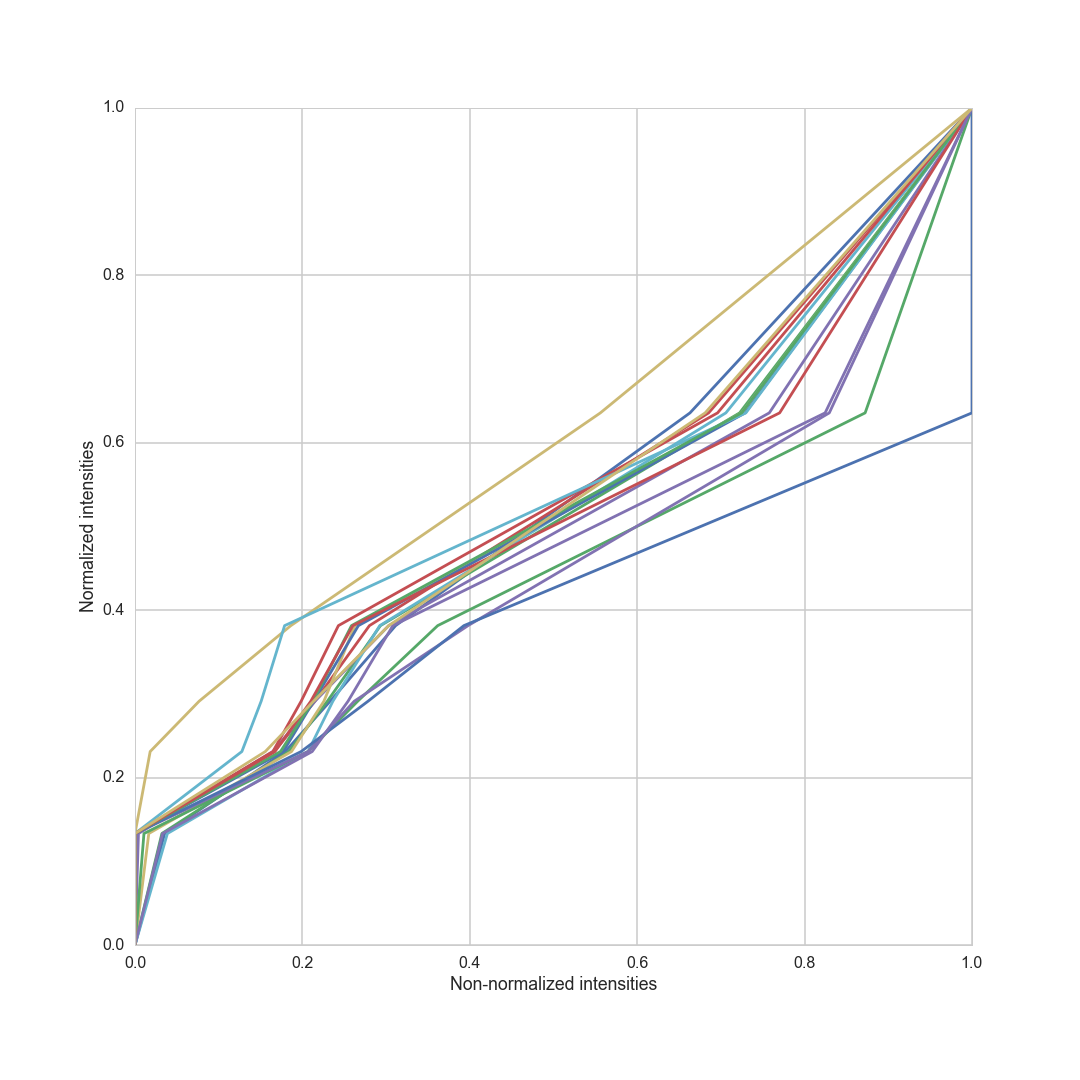
\includegraphics[width=0.4\textwidth]{5_normalization/figures/T2-normalization/piecewise-linear.png}}\hfill
  \subfigure[\acs*{srsf} mapping function.]{
    \label{fig:mapsrsf}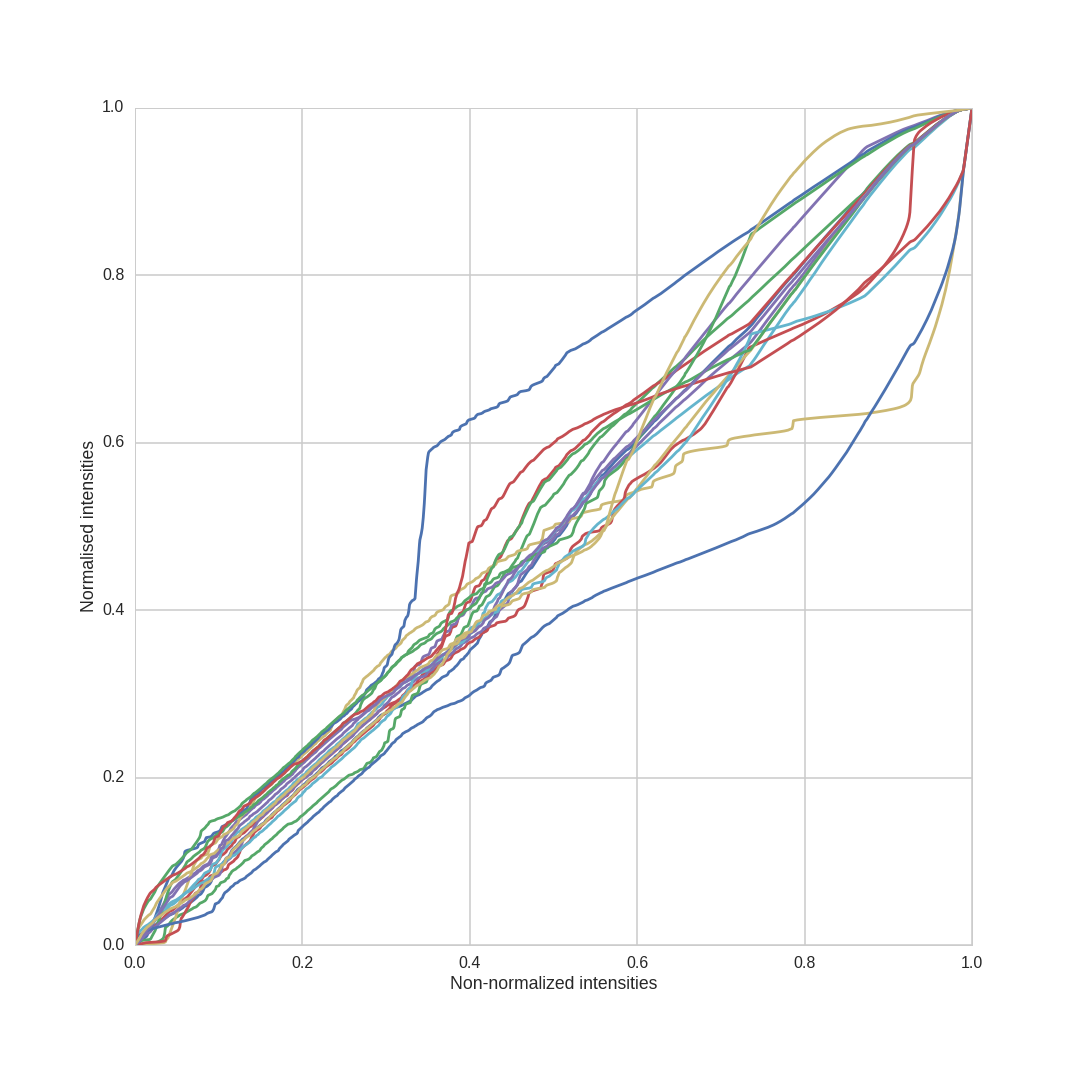
\includegraphics[width=0.4\textwidth]{5_normalization/figures/T2-normalization/srsf.png}}
  \hspace*{\fill}
  \caption[Comparison of the mapping functions found with the piecewise-linear and \acs{srsf}-based normalization.]{Comparison of the mapping functions found with the piecewise-linear and \acs{srsf}-based normalization. Each curve corresponds to a mapping function for a single patient.}
  \label{fig:mapping}
\end{figure}

\Acl{fig}~\ref{fig:qu} depicts the alignment of the different \acp{pdf} using the different methods implemented. 
All the methods seem to address the problem of the \ac{pdf} alignment of the full prostate data.
However, the Rician normalization outperforms the other methods when focusing solely on the \ac{cap} data.
The \ac{pdf} computed in this specific area is more skewed from its original shape in the case of the piecewise-linear normalization than with the 3 other normalization strategies.
The \ac{srsf} normalization gets unstable due to the warping function $\gamma$ found which is in practise non-smooth as shown in \acs{fig}\,\ref{fig:mapsrsf}.

\begin{landscape}

\begin{figure}
  \hspace*{\fill}
  \subfigure[Raw prostate.]{
    \label{subfig:raw}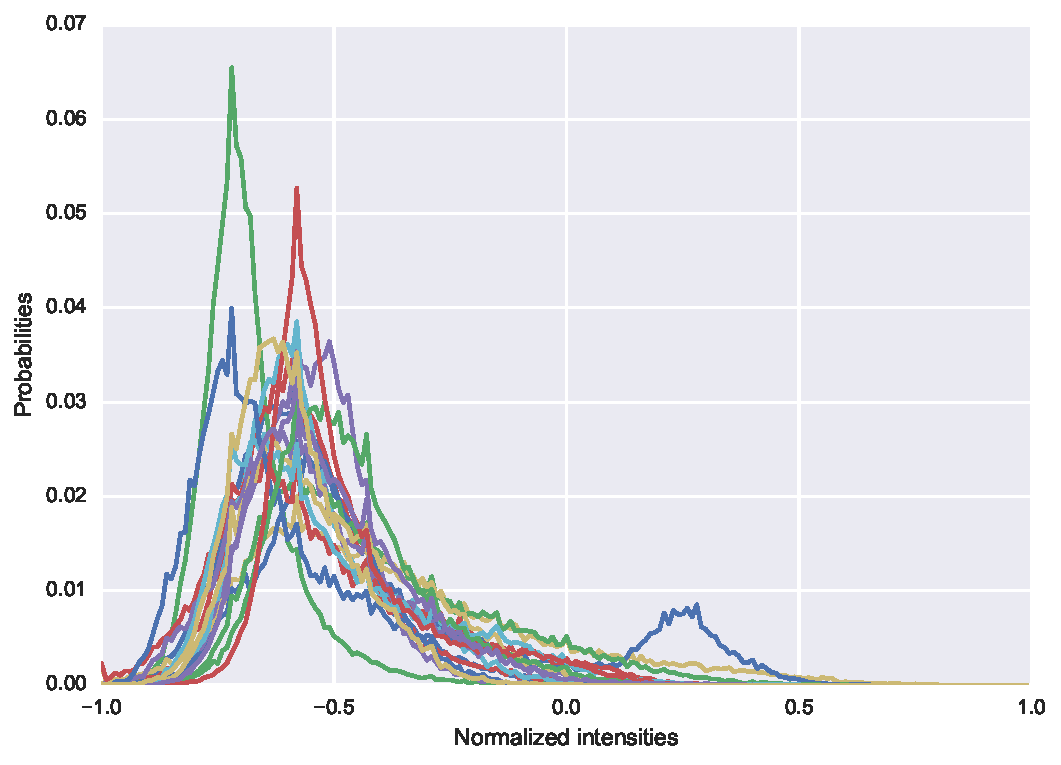
\includegraphics[width=.23\linewidth]{5_normalization/figures/T2-normalization/raw.pdf}}
  \hfill
  \subfigure[Raw \acs*{cap}]{
    \label{subfig:raw_cap}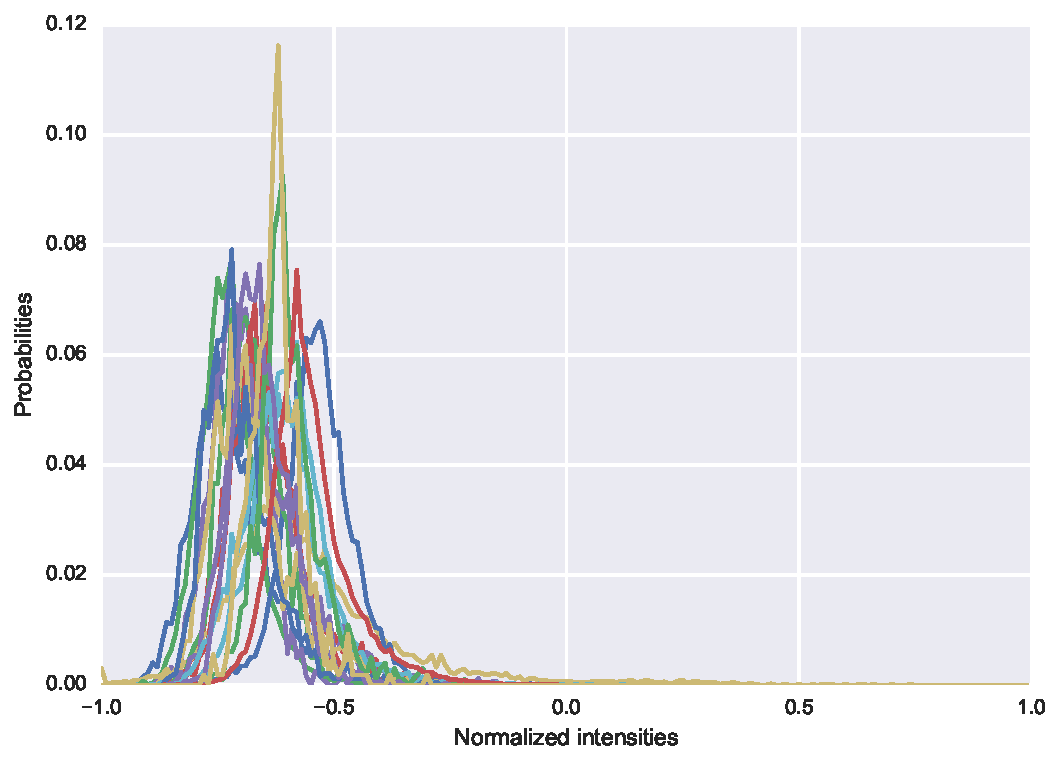
\includegraphics[width=.23\linewidth]{5_normalization/figures/T2-normalization/raw_cap.pdf}}
  \hspace*{\fill}
  \\
  \hspace*{\fill}
  \subfigure[Gaussian prostate.]{
    \label{subfig:gaussian}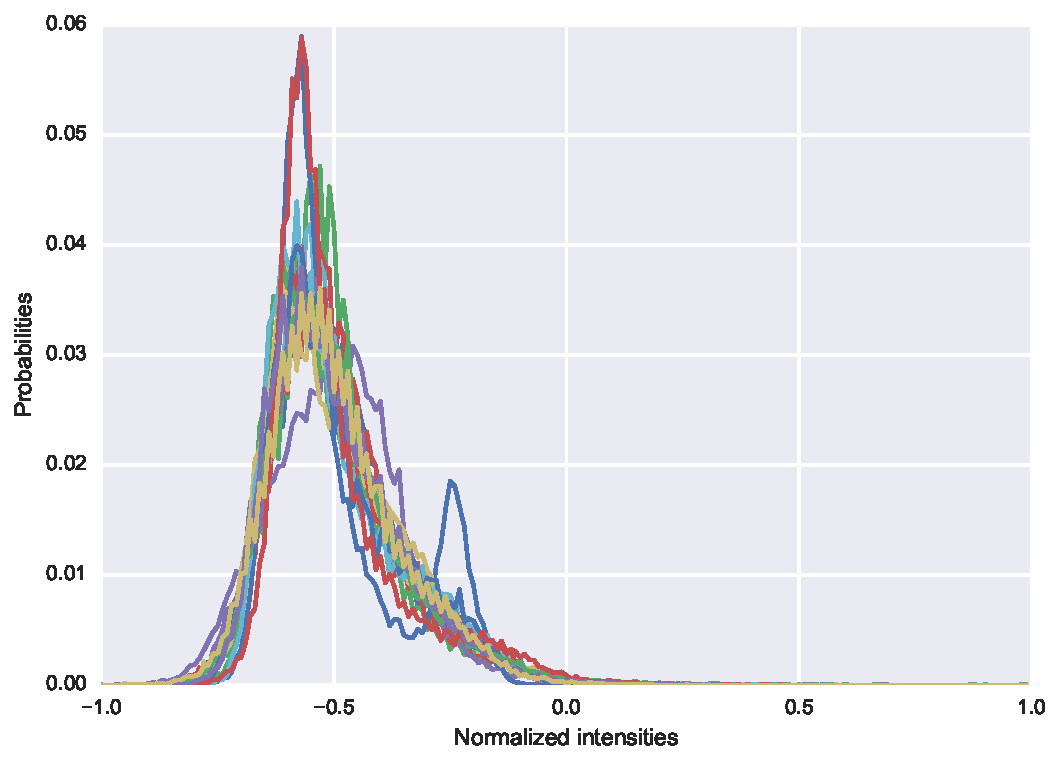
\includegraphics[width=.23\linewidth]{5_normalization/figures/T2-normalization/gaussian.pdf}}
  \hfill
  \subfigure[Rician prostate.]{
    \label{subfig:rician}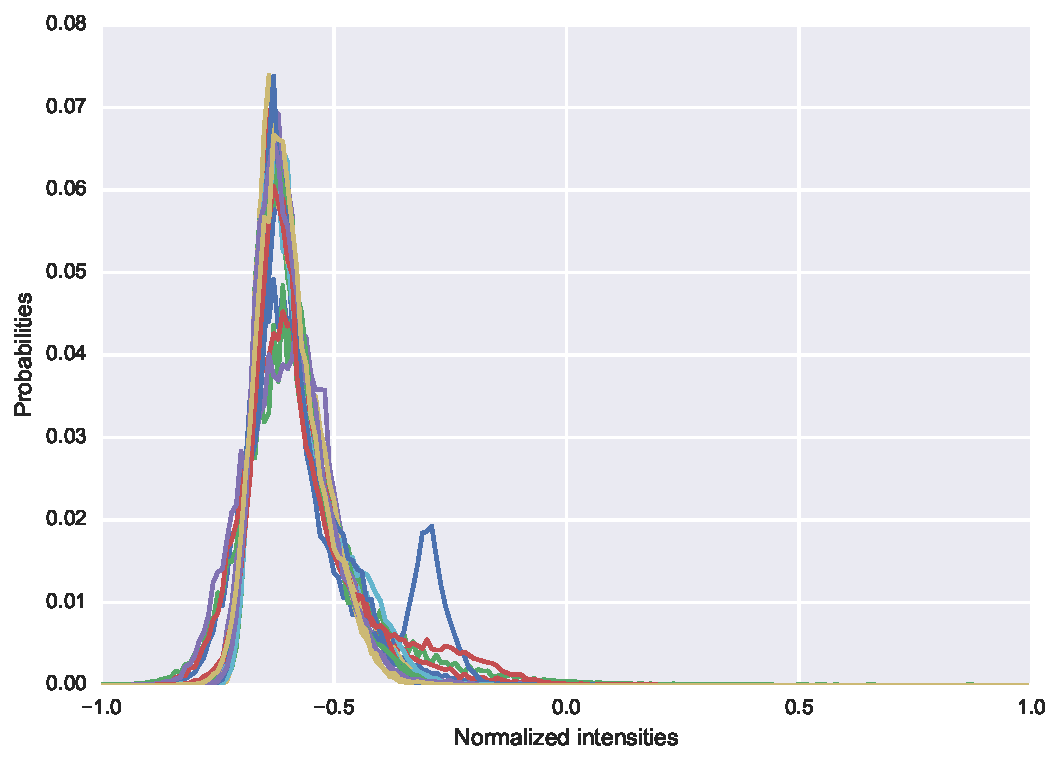
\includegraphics[width=.23\linewidth]{5_normalization/figures/T2-normalization/rician.pdf}}
  \hfill
  \subfigure[Linear prostate.]{
    \label{subfig:piecewise}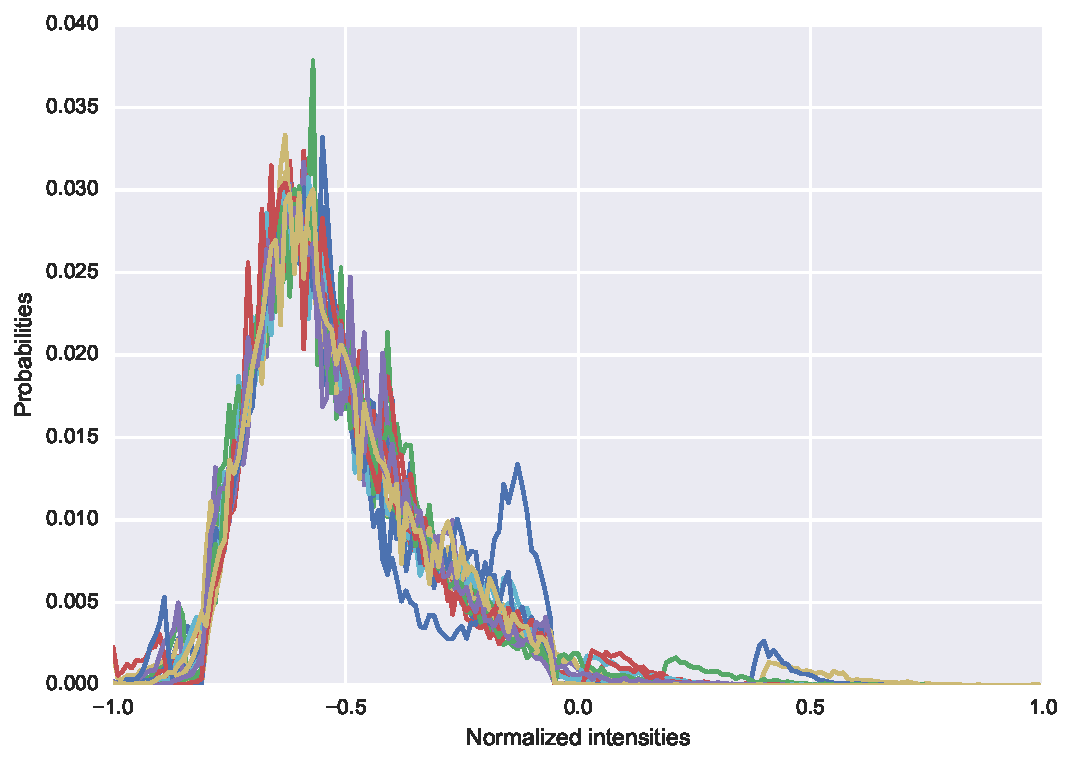
\includegraphics[width=.23\linewidth]{5_normalization/figures/T2-normalization/piecewise.pdf}}
  \hfill
  \subfigure[\acs*{srsf} prostate.]{
    \label{subfig:srsf}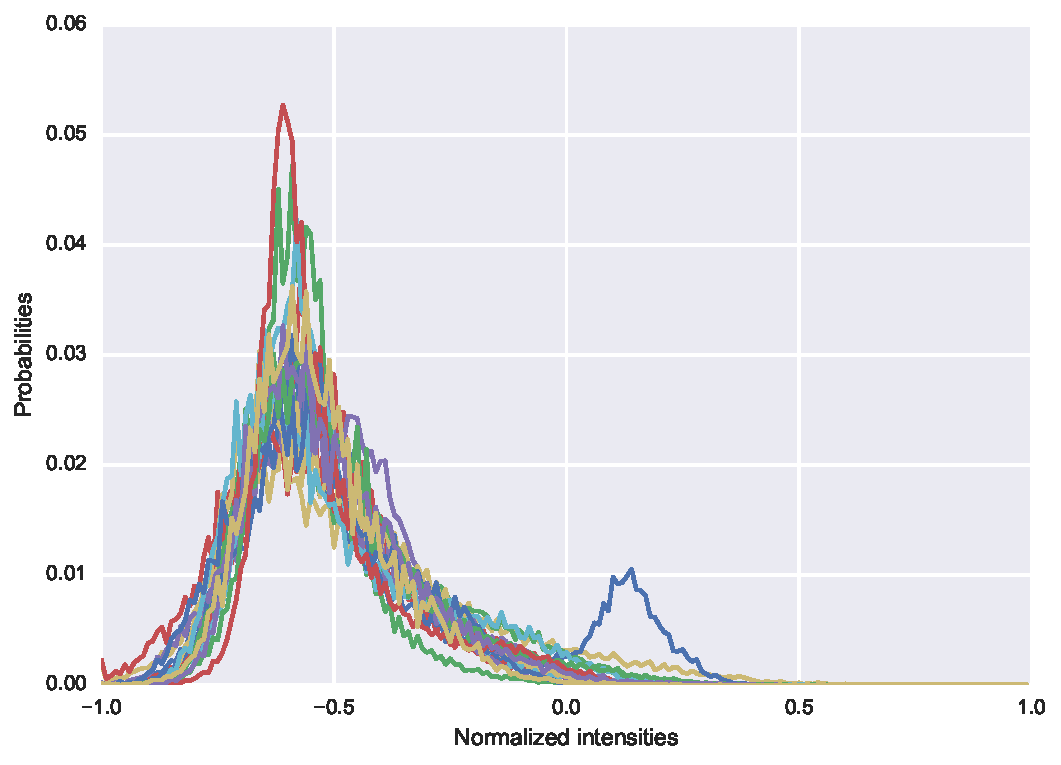
\includegraphics[width=.23\linewidth]{5_normalization/figures/T2-normalization/srsf.pdf}}
  \hspace*{\fill}\\
  \hspace*{\fill}
  \subfigure[Gaussian \acs*{cap}.]{
    \label{subfig:gaussian_cap}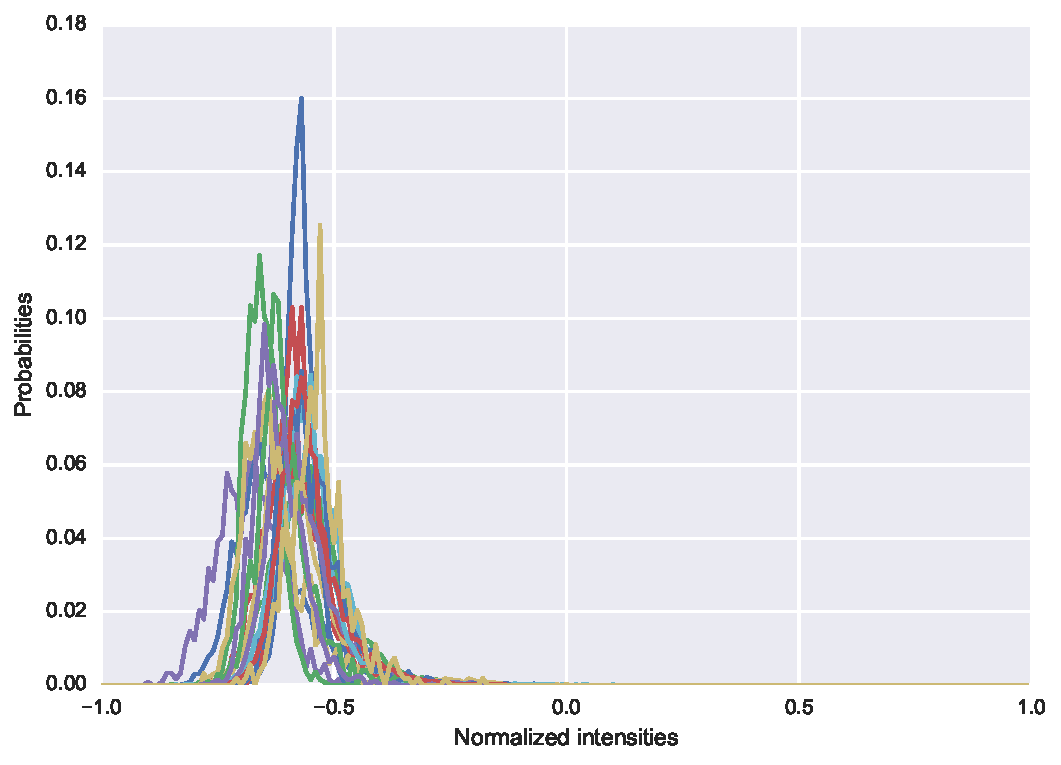
\includegraphics[width=.23\linewidth]{5_normalization/figures/T2-normalization/gaussian_cap.pdf}}
  \hfill
  \subfigure[Rician \acs*{cap}.]{
    \label{subfig:rician_cap}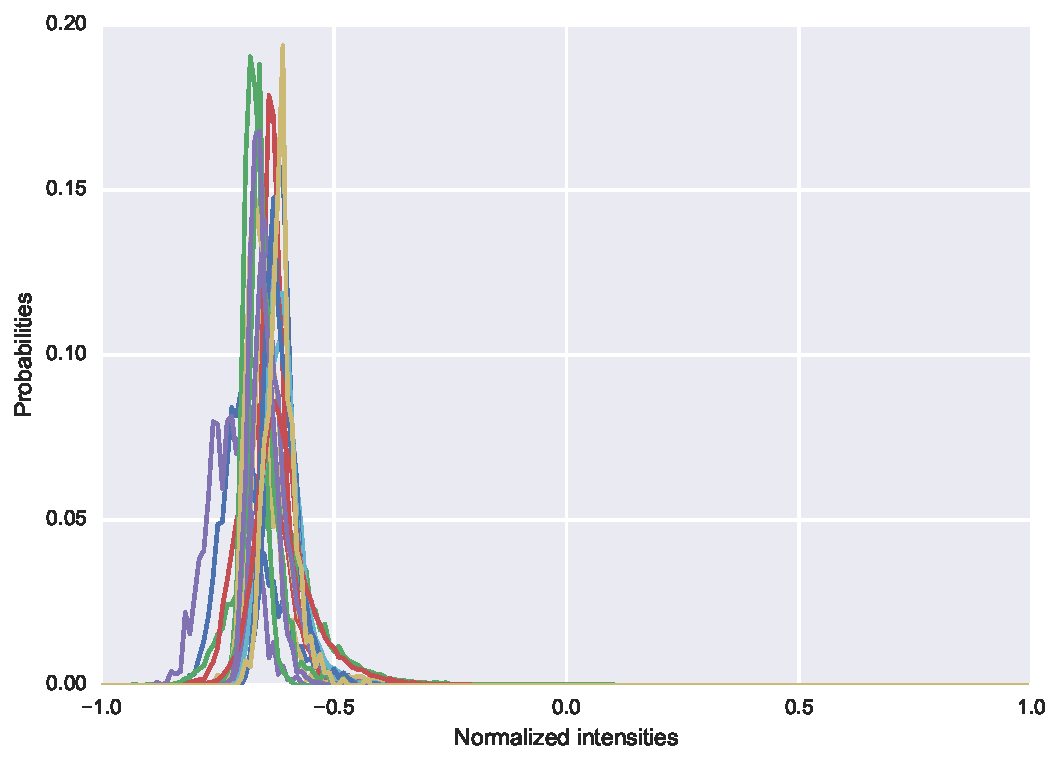
\includegraphics[width=.23\linewidth]{5_normalization/figures/T2-normalization/rician_cap.pdf}}
  \hfill
  \subfigure[Linear \acs*{cap}.]{
    \label{subfig:piecewise_cap}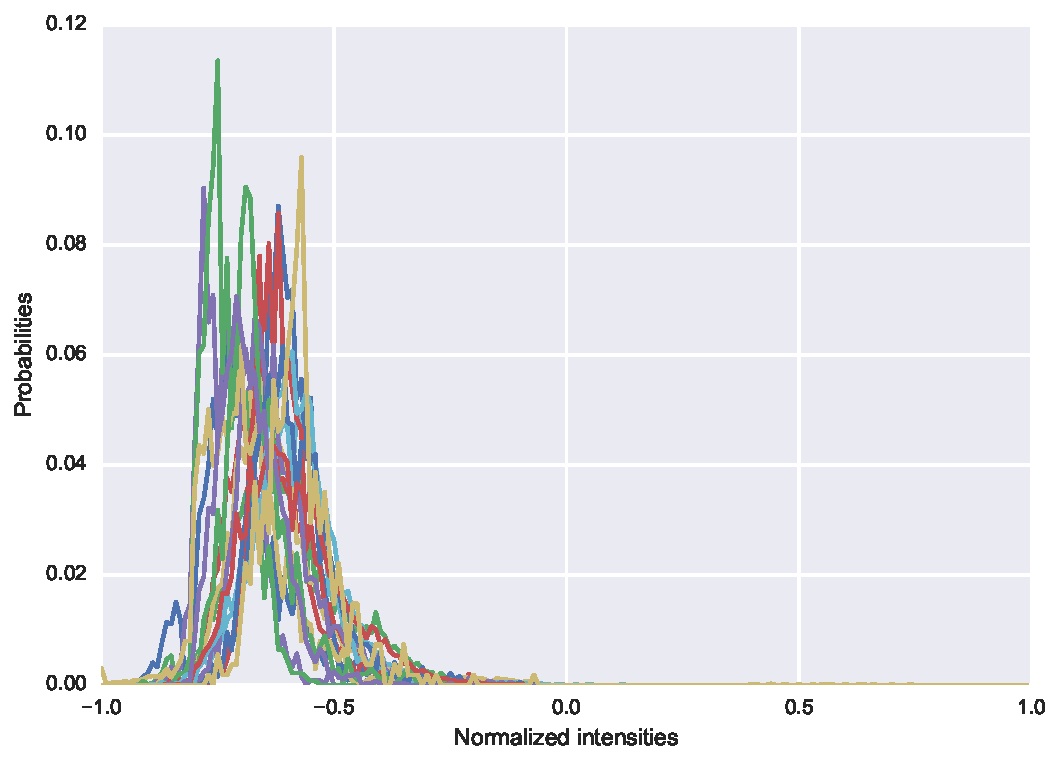
\includegraphics[width=.23\linewidth]{5_normalization/figures/T2-normalization/piecewise_cap.pdf}}
  \hfill
  \subfigure[\acs*{srsf} \acs*{cap}.]{
    \label{subfig:srsf_cap}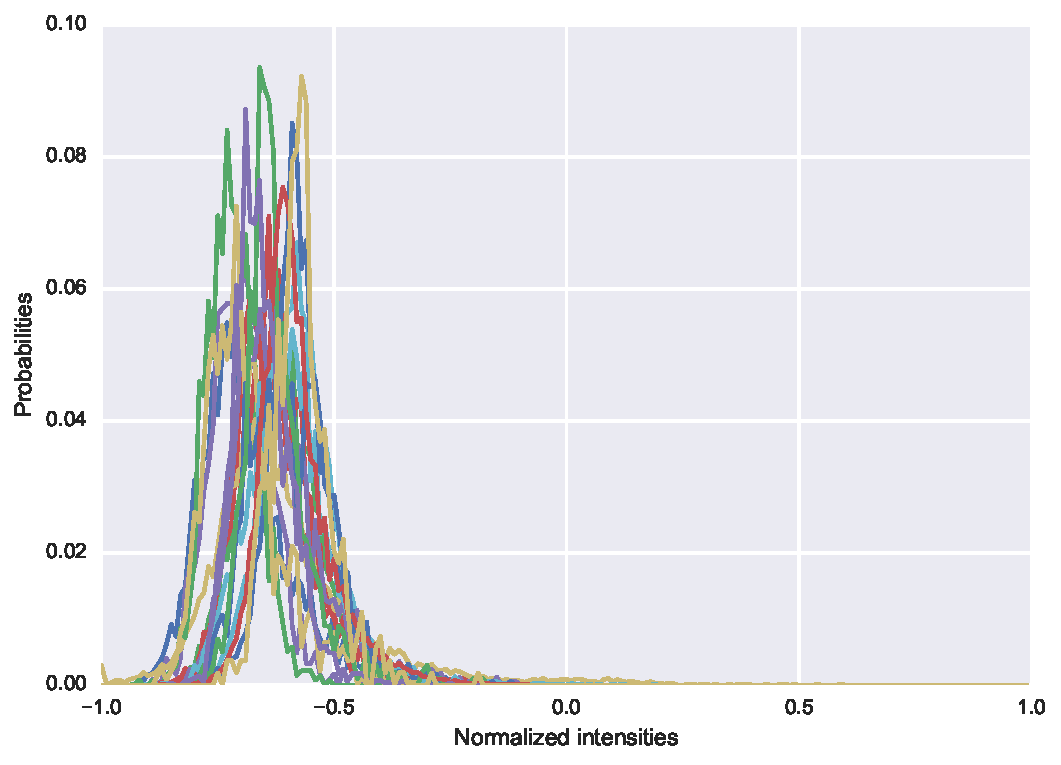
\includegraphics[width=.23\linewidth]{5_normalization/figures/T2-normalization/srsf_cap.pdf}}
  \hspace*{\fill}
  \caption[Qualitative valuation for \acs*{t2w}-\acs*{mri}]{Qualitative evaluation by visual inspection of the alignment of the \acs*{pdf}s for the full prostate and the \acs*{cap} in \acs*{t2w}-\acs*{mri}. The first row corresponds to the original \acs*{pdf}}
  \label{fig:qu}
\end{figure}

\end{landscape}

\paragraph{Quantitative results}

\begin{figure}
  \centering
  \subfigure[]{
    \label{fig:qtfull}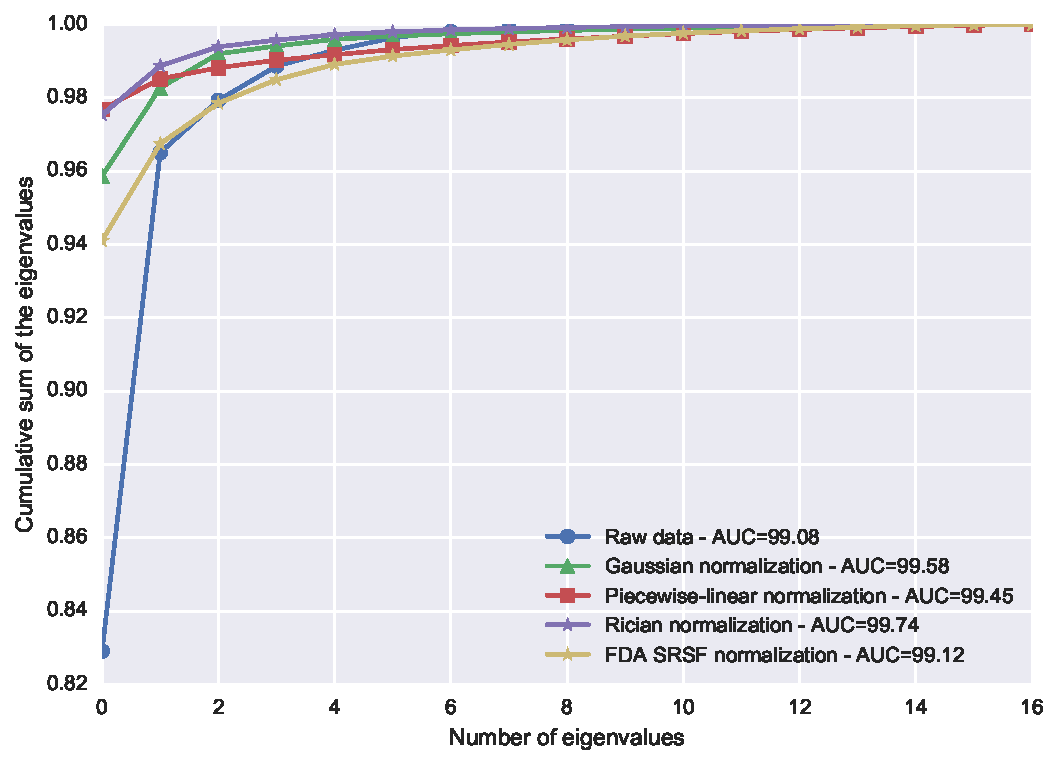
\includegraphics[width=0.8\textwidth]{5_normalization/figures/T2-normalization/quantitative_1.pdf}}\\
  \subfigure[]{
    \label{fig:qtcap}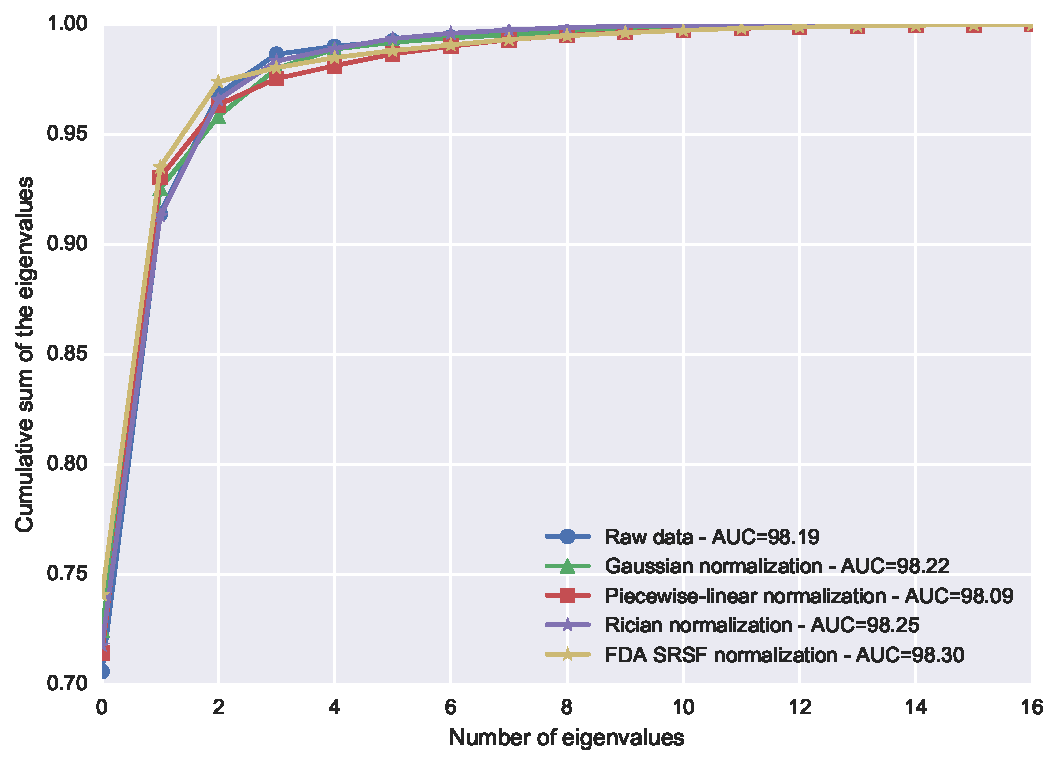
\includegraphics[width=0.8\textwidth]{5_normalization/figures/T2-normalization/quantitative_2.pdf}}
  \caption{Spectral evaluation using \ac{pca} decomposition: \protect\subref{fig:qtfull} evaluation considering the full prostate, \protect\subref{fig:qtcap} evaluation considering only the \ac{cap}.}
  \label{fig:qt}
\end{figure}

In overall, all normalization methods improve the alignment of the \acp{pdf}.
The parametric methods outperform the non-parametric while evaluating the \ac{pdf} alignment considering the full prostate organ.
Furthermore, the Rician normalization is more appropriate than the Gaussian normalization.
The \ac{srsf}-based normalization is shown to perform poorly which might be due to the instability of the mapping function inferred.
However, by focusing on the solely on the \ac{cap} region, the \ac{srsf} outperforms the other methods followed by the Rician normalization.
Therefor, the Rician normalization outperforms the other methods with an \ac{auc} of $99.74$ and $98.25$ considering the full prostate and \ac{cap}, respectively.

\subsection{Conclusion}\label{subsec:chp5:T2-norm:dis-con}
In this section, we propose to normalize the \ac{t2w}-\ac{mri} prostate images using two new strategies: (i) based on a Rician \textit{a priori} and (ii) based on a \ac{srsf} representation.
An extensive comparison has been conducted showing that the Rician normalization outperforms the Gaussian, \ac{srsf}-based, and piecewise-linear normalization for \ac{t2w}-\ac{mri} prostate images normalization.
As avenues for future research, the contribution of the Rician normalization must be evaluated in a classification framework.
Although our proposed evaluation metric seems more appropriate than the previous method, we think that complementary metric should be proposed.
Furthermore, normalized \ac{t2w}-\ac{mri} can be included with other modalities in order to perform classification using \ac{mpmri} data.